% A LaTeX template for EXECUTIVE SUMMARY of the MSc Thesis submissions to
% Politecnico di Milano (PoliMi) - School of Industrial and Information Engineering
%
% P. F. Antonietti, S. Bonetti, A. Gruttadauria, G. Mescolini, A. Zingaro
% e-mail: template-tesi-ingind@polimi.it
%
% Last Revision: October 2021
%
% Copyright 2021 Politecnico di Milano, Italy. Inc. All rights reserved.

\documentclass[11pt,a4paper]{article}

%------------------------------------------------------------------------------
%	REQUIRED PACKAGES AND  CONFIGURATIONS
%------------------------------------------------------------------------------
% PACKAGES FOR TITLES
\usepackage{titlesec}
\usepackage{color}

% PACKAGES FOR LANGUAGE AND FONT
\usepackage[utf8]{inputenc}
\usepackage[english]{babel}
\usepackage[T1]{fontenc} % Font encoding

% PACKAGES FOR IMAGES
\usepackage{graphicx}
\graphicspath{{Images/}} % Path for images' folder
\usepackage{eso-pic} % For the background picture on the title page
\usepackage{subfig} % Numbered and caption subfigures using \subfloat
\usepackage{caption} % Coloured captions
\usepackage{transparent}

% STANDARD MATH PACKAGES
\usepackage{amsmath}
\usepackage{amsthm}
\usepackage{bm}
\usepackage[overload]{empheq}  % For braced-style systems of equations

% PACKAGES FOR TABLES
\usepackage{tabularx}
\usepackage{longtable} % tables that can span several pages
\usepackage{colortbl}

% PACKAGES FOR ALGORITHMS (PSEUDO-CODE)
\usepackage{algpseudocode}
\usepackage{algorithm}
% PACKAGES FOR REFERENCES & BIBLIOGRAPHY
\usepackage[colorlinks=true,linkcolor=black,anchorcolor=black,citecolor=black,filecolor=black,menucolor=black,runcolor=black,urlcolor=black]{hyperref} % Adds clickable links at references
\usepackage{cleveref}
\usepackage[square, numbers, sort&compress]{natbib} % Square brackets, citing references with numbers, citations sorted by appearance in the text and compressed
\bibliographystyle{plain} % You may use a different style adapted to your field

% PACKAGES FOR THE APPENDIX
\usepackage{appendix}

% PACKAGES FOR ITEMIZE & ENUMERATES
\usepackage{enumitem}

% OTHER PACKAGES
\usepackage{amsthm,thmtools,xcolor} % Coloured "Theorem"
\usepackage{comment} % Comment part of code
\usepackage{fancyhdr} % Fancy headers and footers
\usepackage{lipsum} % Insert dummy text
\usepackage{tcolorbox} % Create coloured boxes (e.g. the one for the key-words)
\usepackage{stfloats} % Correct position of the tables
\DeclareMathOperator*{\argmin}{arg\,min}
\usepackage{relsize}
\usepackage{amsfonts}


%-------------------------------------------------------------------------
%	NEW COMMANDS DEFINED
%-------------------------------------------------------------------------
% EXAMPLES OF NEW COMMANDS -> here you see how to define new commands
\newcommand{\bea}{\begin{eqnarray}} % Shortcut for equation arrays
\newcommand{\eea}{\end{eqnarray}}
\newcommand{\e}[1]{\times 10^{#1}}  % Powers of 10 notation
\newcommand{\mathbbm}[1]{\text{\usefont{U}{bbm}{m}{n}#1}} % From mathbbm.sty
\newcommand{\pdev}[2]{\frac{\partial#1}{\partial#2}}

% NB: you can also override some existing commands with the keyword \renewcommand

%----------------------------------------------------------------------------
%	ADD YOUR PACKAGES (be careful of package interaction)
%----------------------------------------------------------------------------


%----------------------------------------------------------------------------
%	ADD YOUR DEFINITIONS AND COMMANDS (be careful of existing commands)
%----------------------------------------------------------------------------


% Do not change Configuration_files/config.tex file unless you really know what you are doing.
% This file ends the configuration procedures (e.g. customizing commands, definition of new commands)
% Set the geometric layout of the document
\usepackage{geometry}
\geometry{
  top=3cm,
  left = 2.0cm,
  right = 2.0cm,
  bottom=2cm,
  headheight= 2cm,
  headsep= 0cm,
}
\raggedbottom

% Create color bluePoli (-> manuale grafica coordinata:  https://www.polimi.it/fileadmin/user_upload/il_Politecnico/grafica-coordinata/2015_05_11_46xy_manuale_grafica_coordinata.pdf)
\definecolor{bluePoli}{cmyk}{0.4,0.1,0,0.4}

% Custom theorem environments
\declaretheoremstyle[
  headfont=\color{bluePoli}\normalfont\bfseries,
  bodyfont=\color{black}\normalfont\itshape,
]{colored}

\captionsetup[figure]{labelfont={color=bluePoli}} % Set colour of the captions
\captionsetup[table]{labelfont={color=bluePoli}} % Set colour of the captions
\captionsetup[algorithm]{labelfont={color=bluePoli}} % Set colour of the captions

\theoremstyle{colored}
\newtheorem{theorem}{Theorem}[section]
\newtheorem{proposition}{Proposition}[section]

% Enhances the features of the standard "table" and "tabular" environments.
\newcommand\T{\rule{0pt}{2.6ex}}
\newcommand\B{\rule[-1.2ex]{0pt}{0pt}}

% Algorithm description
\newcounter{algsubstate}
\renewcommand{\thealgsubstate}{\alph{algsubstate}}
\newenvironment{algsubstates}{
    \setcounter{algsubstate}{0}%
    \renewcommand{\STATE}{%
    \stepcounter{algsubstate}%
    \Statex {\small\thealgsubstate:}\space}
    }{}

% Custom theorem environment
\newcolumntype{L}[1]{>{\raggedright\let\newline\\\arraybackslash\hspace{0pt}}m{#1}}
\newcolumntype{C}[1]{>{\centering\let\newline\\\arraybackslash\hspace{0pt}}m{#1}}
\newcolumntype{R}[1]{>{\raggedleft\let\newline\\\arraybackslash\hspace{0pt}}m{#1}}

% Custom itemize environment
\setlist[itemize,1]{label=$\bullet$}
\setlist[itemize,2]{label=$\circ$}
\setlist[itemize,3]{label=$-$}
\setlist{nosep}

% Set separation of columns
\setlength{\columnsep}{30pt}

% Create command for background pic
\newcommand\BackgroundPic{% Adding background picture
	\put(230,358){
		\parbox[b][\paperheight]{\paperwidth}{%
			\vfill
			\centering
			\transparent{0.4}
			
\includegraphics[width=0.5\paperwidth]{raggiera_polimi.eps}%
			\vfill
}}}

% Set indentation
\setlength\parindent{0pt}

% Custom title commands
\titleformat{\section}
{\color{bluePoli}\normalfont\Large\bfseries}
{\color{bluePoli}\thesection.}{1em}{}
\titlespacing*{\section}
{0pt}{2ex}{1ex}

\titleformat{\subsection}
{\color{bluePoli}\normalfont\large\bfseries}
{\color{bluePoli}\thesubsection.}{1em}{}
\titlespacing*{\subsection}
{0pt}{2ex}{1ex}

% Custom headers and footers
\pagestyle{fancy}
\fancyhf{}

\fancyfoot{}
\fancyfoot[C]{\thepage} % page
\renewcommand{\headrulewidth}{0mm} % headrule width
\renewcommand{\footrulewidth}{0mm} % footrule width

\makeatletter
\patchcmd{\headrule}{\hrule}{\color{black}\hrule}{}{} % headrule
\patchcmd{\footrule}{\hrule}{\color{black}\hrule}{}{} % footrule
\makeatother

% -> Create the header
\chead[C]{
\centering
\begin{tcolorbox}[arc=0pt, boxrule=0pt, colback=bluePoli!60, width=\textwidth, colupper=white]
    \textbf{Homework 1} \hfill \textbf{\author}  
\end{tcolorbox}
}


% Insert here the info that will be displayed into your Title page
% -> title of your work
\renewcommand{\title}{Homework 1}
% -> author name and surname
\renewcommand{\author}{Federica Botta, Simone Colombara and Michele Di Sabato}
% -> MSc course
\newcommand{\course}{Scientific computing tools for advanced mathematical modelling}
% -> advisor name and surname
%\newcommand{\advisor}{Dr. Stefano Pagani}
% IF AND ONLY IF you need to modify the co-supervisors you also have to modify the file Configuration_files/title_page.tex (ONLY where it is marked)
%\newcommand{\firstcoadvisor}{Name Surname} % insert if any otherwise comment
%\newcommand{\secondcoadvisor}{Name Surname} % insert if any otherwise comment
% -> academic year
\newcommand{\YEAR}{2021-2022}

%-------------------------------------------------------------------------
%	BEGIN OF YOUR DOCUMENT
%-------------------------------------------------------------------------
\begin{document}

%-----------------------------------------------------------------------------
% TITLE PAGE
%-----------------------------------------------------------------------------
% Do not change Configuration_files/TitlePage.tex (Modify it IF AND ONLY IF you need to add or delete the Co-advisors)
% This file creates the Title Page of the document
% DO NOT REMOVE SPACES BETWEEN LINES!

%\twocolumn[{\begin{@twocolumnfalse}

\AddToShipoutPicture*{\BackgroundPic}

\hspace{-0.6cm}
\includegraphics[width=0.6\textwidth]{logo_polimi_ing_indinf.eps}

\vspace{-1mm}
\fontsize{0.3cm}{0.5cm}\selectfont \bfseries \textsc{\color{bluePoli} Homework report}\\

\vspace{-0.2cm}
\Large{\textbf{\color{bluePoli}{\title}}}\\

\vspace{-0.2cm}
\fontsize{0.3cm}{0.5cm}\selectfont \bfseries \textsc{\color{bluePoli} \course}\\

\vspace{-0.2cm}
\fontsize{0.3cm}{0.5cm} \selectfont \bfseries Authors: \textsc{\textbf{\author}}\\

%\vspace{-0.4cm}
%\fontsize{0.3cm}{0.5cm}\selectfont \bfseries Advisor: \textsc{\textbf{\advisor}}\\

% if only ONE co-advisor is present:
%\vspace{-0.4cm}
%\fontsize{0.3cm}{0.5cm}\selectfont \bfseries Co-advisor: \textsc{\textbf{\firstcoadvisor}}\\
% if more than one co-advisors are present:
%\vspace{-0.4cm}
%\fontsize{0.3cm}{0.5cm}\selectfont \bfseries Co-advisors: \textsc{\textbf{\firstcoadvisor}}\textsc{\textbf{\secondcoadvisor}}\\

\vspace{-0.4cm}
\fontsize{0.3cm}{0.5cm}\selectfont \bfseries Academic year: \textsc{\textbf{\YEAR}}

\small \normalfont

\vspace{11pt}

\centerline{\rule{1.0\textwidth}{0.4pt}}

%\vspace{15pt}
%\end{@twocolumnfalse}}]

\thispagestyle{plain} % In order to not show the header in the first page


%%%%%%%%%%%%%%%%%%%%%%%%%%%%%%
%%     THESIS MAIN TEXT     %%
%%%%%%%%%%%%%%%%%%%%%%%%%%%%%%

%-----------------------------------------------------------------------------
% INTRODUCTION
%-----------------------------------------------------------------------------
\section{Mathematical formulation of the problem}\label{sec:introduction}

The framework of this project is the following: the normal diffusion of the differential potential in the heart is hindered by a re-entry of the signal, possibly caused by scar tissue in specific areas of the heart. This problem could cause an arrhythmia, which could be fatal. In order to restore the normal diffusion of the potential through the affected region, an Anti-Tachycardia Pacing (ATP) device is inserted, its purpose is to deliver an impulse to avoid the re-entry.\newline
We are given three ECG signals observed for 450 ms of three different patients and a numerical solver to compute an approximation of an ECG. The goal of this project is to calibrate the Rogers-McCulloch model for the ionic current and the ATP strategy:
\vspace{1mm}
\begin{itemize}\setlength\itemsep{1.5mm}
    \item $\nu_2$: Rogers-McCulloch model parameter, which ranges in (0.0116, 0.0124)
    \item $t_s$: starting time of the shock, which ranges in (450 ms, 525 ms)
    \item $\Delta t_{s}$: duration of the shock. To maximize the duration of the battery it's best to keep this parameter below 10 milliseconds and possibly as small as possible.
\end{itemize}
\vspace{1mm}
Moreover, these parameters need to be patient-specific.\vspace{1mm}\\
\noindent To calibrate $\nu_2$, we have to compare the exact solutions with our numerical solutions for each patient, considering the problem without the intervention of the ATP device (until 450 ms). Instead, the "best" $t_{s}$ and $\Delta t_{s}$ are the ones that lead to an ECG equal to zero in the tracking window (600 ms, 800 ms).\\
The underlying model is the monodomain problem coupled with the Rogers-McCulloch ionic model which gives an estimation of the total ionic current ($I_{ion}$) and its gradient ($g$), being:
    \begin{equation}\label{model}
	\begin{cases}
	I_{ion}(U_t, W_t) = \nu_0 U_t (1-\frac{U_t}{v_{th}})(1-\frac{U_t}{v_pk})+\nu_1 U_t W_t,
	\\
	\vspace{2mm}
	g(U_t, W_t) = \nu_2 (\frac{U_t}{v_{pk}}-\nu_3 W_t).
	\end{cases}
    \end{equation}
Where $U_t$ is the transmembrane potential and $W_t$ is the unique gating variable. Note that the parameter $\nu_2$ is used in this model.\newline
We define the signals output during the time evolution (pseudo or numerical ECG) as $u(t)$ (without the presence of ATP device), having the exact signals of the three patients $u_{ex}(t)$ the problem for finding $\nu_2$ becomes:
    \begin{equation}\label{nu2}
    \text{find $\nu_{2}^{*}$= } \argmin\limits_{\nu_2} \Vert u(t)-u_{ex}(t) \Vert_{MSE}  \quad \forall t \in (0,450) \quad  ms.
    \end{equation}
Instead, to find $t_{s}$ and $\Delta t_{s}$ we use the $\nu_2$ value found from equation (\ref{nu2}) for each subject and, this time, we also take into account the effect of the impulse from the ATP device. The mathematical formulation of the problem is\footnote{we also tried using " $+ \lambda (\Delta t_s)^2$ " instead of " $+ \lambda \Delta t_s$ "}:

    \begin{equation} \label{min_proc}
        \textrm{find }(t_{s}^{*}, \Delta t _{s}^{*}):= \argmin\limits_{(t_s, \Delta t_s)} (\Vert u(t)-0 \Vert_{MSE} + \lambda \Delta t_s) \qquad \forall t \in (600,800)ms.
    \end{equation}
The first term aims at reaching a signal equal to 0 on the entire the tracking window and the term involving $\lambda$ is used to penalize large impulse durations, which undermine the device's battery.
\section{Methods}
\label{sec:methods}
\subsection{Algorithm for $\nu_2$}\label{alg_nu}
We use a modified random search, based on adapting the standard deviation of the normal distribution, to solve equation (\ref{nu2}):
\begin{algorithm}
\caption{Algorithm for $\nu_2$ - Adaptive Random Search}
\begin{algorithmic} 
\For{each patient}
\State $\nu_{2,best} = 0.012$ \Comment{Initially set $\nu_2$ as the mid value}
\vspace{1mm}
\State $\texttt{MSE}_{best}$ = \textbf{MSE}$(u_{num}(\nu_{2,best}), u_{ex}^{denoised})$
\vspace{1mm}
\While{ $\texttt{it} \leq \texttt{it}_{max}$}
\vspace{1mm}
   \If{$\texttt{it} \leq 10$} 
   \vspace{1mm}
    \State $\nu_{2,guess} = \nu_{2,best}+0.004 \cdot \mathcal{N}(0,1)$ \Comment{Burn-in iterations with fixed variance}
    \vspace{1mm}
    \Else
    \vspace{1mm}
    \State $\nu_{2,guess} = \nu_{2,best}+0.004 \ \frac{(\texttt{it}_{max}-it)}{\texttt{\texttt{it}}_{max}-10}  \cdot \mathcal{N}(0,1)$ \Comment{Decreasing variance}
    \vspace{1mm}
\EndIf
\vspace{1mm}
\State $\texttt{MSE}_{guess}$ = \textbf{MSE}$(u_{num}(\nu_{2,guess}), u_{ex}^{denoised})$
\vspace{1mm}
\If{$\texttt{MSE}_{guess} \leq \texttt{MSE}_{best}$}
\vspace{1mm}
\State $\texttt{MSE}_{best}=\texttt{MSE}_{guess}$
\vspace{1mm}
\State $\nu_{2,best}=\nu_{2,guess}$
\vspace{1mm}
\EndIf
\vspace{1mm}
\EndWhile
\vspace{1mm}
\State Final estimation for the current patient is $\nu_{2,best}$ with $\texttt{MSE}_{best}$
\vspace{1mm}
\EndFor
\end{algorithmic}
\smaller 
\vspace{0.3cm}
\textbf{Remark}: $u_{ex}^{denoised}(\nu)$ stands for the denoised exact solution and $u_{num}(\nu)$ for the numerical one. \normalsize \\
\smaller \textbf{Remark}: For each iteration, the extraction of $\nu_{2,guess}$ is repeated until it falls in the range (0.0116, 0.0124), to avoid exceeding the bounds for this parameter. \normalsize
\end{algorithm}

\noindent
Note that:
\begin{itemize}
    \item It's a variation of the random search method because after some loops the variance is reduced according to the number of iterations;
    \item The MSE is computed using the difference between the numerical solution and the exact one, but the latter is denoised using a bandpass filter;
    \item We decided to set $\texttt{it}_{max}$ = 20 in order to keep the computational load low.
\end{itemize}

\subsection{Algorithm for $\Delta t_{s}^{*}$ and $t_{s}^{*}$}\label{alg_t}
Once the parameter $\nu_2$ has been calibrated, to find the duration and timing of the shock, a simple random grid search carried out on the loss function defined in equation (\ref{min_proc}) is too expensive, since it requires knowing the numerical ECG for each patient and for each choice of $(t_s, \Delta t_s)$. Instead, we opted for a Bayesian approach, which consists in using a Bayesian Optimization algorithm, used to find the maximum of an objective function $f$ whenever evaluating $f$ itself is costly (financially or, as in our case, computationally). We relied on the articles \cite{bayesopt_1} and \cite{bayesopt_2}. \newline
The core idea of Bayesian Optimization is that the objective function $f$ is modeled a priori as a Gaussian Process, which is updated whenever new evaluations of $f$ are available (thus obtaining the posterior distribution of $f$, which is proven to be still a Gaussian Process). Suppose that we already have collected $n$ points in the dataset $\mathcal{D}_{1:n} = \{\boldsymbol{x}_1,...,\boldsymbol{x}_n\}$ on which we know the value of $f$: $f(\boldsymbol{x}_i) = f_i \ \forall i = 1,...,n$. To select the $(n+1)$-th point, the algorithm chooses the one which is "most likely" to yield a higher value of $f$ than the ones already at our disposal in our dataset $\mathcal{D}_{1:n}$. In the algorithm, the phrase "most likely" is quantified in the following way:
\begin{equation} \label{acqfunc}
    \boldsymbol{x}_{n+1} = \textrm{argmax}_{\boldsymbol{x}} \{u(\boldsymbol{x})\}
\end{equation}
where $u$ is called acquisition function. For our project, we tried using two kinds of acquisition functions:\\
defining $f_{n}^{*} \overset{\operatorname{def}}{=} \textrm{argmax}_{i  \in  [1,n]} f(\boldsymbol{x}_{i})$,
\begin{itemize}
    \item Probability of Improvement: $u(\boldsymbol{x}) = \text{I\kern-0.15em P}(f(\boldsymbol{x})\ge f_{n}^{*})=\Phi\biggl({\mu(\boldsymbol{x})-f_{n}^{*}\over \sigma(\boldsymbol{x})}\biggl)$
    \item Expected Improvement: $u(\boldsymbol{x}) = \mathbb{E}_{n}[\textrm{max}\{0, \  f(\boldsymbol{x})-f_{n}^{*}\}]$
\end{itemize}
\vspace{1mm}
The computation of both these functions is based on the assumption that $f$ is modeled as a Gaussian Process. Finally, for our purpose we tried using the following objective functions and since our task is a minimization procedure, we set:
\begin{equation*}
    f(t_s, \Delta t_s) = - \big( \Vert u(t)-0 \Vert_{MSE} + \lambda \Delta t_s \big)
\end{equation*}
\begin{equation*}
    f(t_s, \Delta t_s) = - \big( \Vert u(t)-0 \Vert_{MSE} + \lambda (\Delta t_s)^2 \big)
\end{equation*}
We report the most general form of a Bayesian Optimization algorithm:
\begin{algorithm}[H]
\caption{Bayesian Optimization Algorithm}
\begin{algorithmic}
\For{n = 1, \ldots, N}
\vspace{1mm}
     \State Find the new point $\boldsymbol{x}_{n+1}$ by maximizing the acquisition function $u$: $\boldsymbol{x}_{n+1} = \textrm{argmax}_{ \boldsymbol{x} \in A} u(\boldsymbol{x} \vert \mathcal{D}_{1:n})$
    \vspace{1mm}
    \State Evaluate the objective function $f$ in the new point $\boldsymbol{x}_{n+1}$ and set $f_{n+1} := f(\boldsymbol{x}_{n+1})$
    \vspace{1mm}
    \State Augment the dataset: $\mathcal{D}_{1:n+1} = \{ \mathcal{D}_{1:n}, (\boldsymbol{x}_{n+1}, f_{n+1})\}$
    \vspace{1mm}
    \State Compute the posterior mean $\mu( \cdot \vert \mathcal{D}_{1:n+1} )$ and posterior variance $\sigma^{2}(\cdot \vert \mathcal{D}_{1:n+1})$
    \vspace{1mm}
\EndFor
\end{algorithmic}
\smaller
\vspace{0.3cm}
\textbf{Remark:} $A$ is the parameter space.\\
\textbf{Remark:} $\boldsymbol{x}$ is replaced by the couple $(t_s, \Delta t_s)$
\normalsize
\end{algorithm}
\subsection{Implementation}
In the following list we report the most important functions in our repository, briefly explaining their content and describing some implementation details:
\vspace{1mm}
\begin{itemize}
    \item[-] \texttt{TF2D-nu-2.py}: a modified version of the numerical solver adapted so that it receives as input $\nu_2$.
    \vspace{1mm}
    \item[-] \texttt{solver-ATP.py}: a modified version of the numerical solver adapted so that it receives as input the couple $(t_s, \Delta t_s)$.
    \vspace{1mm}
    \item[-] \color{blue} \texttt{nu2-calibration.py} \color{black}: performs real ECG denoising, applies adaptive random search to tune $\nu_2$ and saves the results in a dedicated directory.
    \vspace{1mm}
    \item[-] \texttt{find-best-savings.py}: returns the best values for parameter $\nu_2$ for the three different patients.
    \vspace{1mm}
    \item[-] \color{blue} \texttt{BayesOpt-impulse-calibration.py} \color{black}: computes 50 Bayesian Optimization steps, following 7 steps of pure random exploration. After finishing the exploration, the script saves the plot of the ECG for each patient and displays the impulse time and duration corresponding to the lowest value of the loss function. 50 iterations is an exaggerated number, as the algorithm consistently proposes a satisfactory couple in roughly 15 iterations.
    \vspace{1mm}
    \item[-] \color{black} \texttt{results-analysis.py}: groups all the $\nu_2$ parameters and their respective MSE obtained through Algorithm 1 and plots them for each patient.
\end{itemize}
\vspace{1mm}
The \color{blue} blue \color{black} scripts are the ones that need to be run in order to obtain the main results. Also, we used some functions from the library \cite{baysopt_git}.\\
Throughout the execution of the calibration, we noticed a recurring pattern, especially evident for the third patient: if we want to obtain a $L^2$ norm of the ECG in the tracking window small enough to annihilate the ECG signal, $\Delta t_s$ ended up being quite high (especially for patient 3). Vice versa, if we tried to penalize a high $\Delta t_s$ using a high value of $\lambda$, either the ECG did not reach zero at all or it reached zero much more slowly than the case with high $\Delta t_s$.
The following list shows the final values for $\lambda$ and the loss function used for the different patients (P1: Patient 1, P2: Patient 2, P3: Patient 3):
\begin{itemize}
    \item [P1:] $L^2 \textrm{ norm in the tracking window} + \lambda (\Delta t_s)^2$, $\lambda = 1$ 
    \item [P2:] $L^2 \textrm{ norm in the tracking window} + \lambda (\Delta t_s)^2$, $\lambda = 1$ 
    \item [P3:] $L^2 \textrm{ norm in the tracking window} + \lambda \Delta t_s$, $\lambda = 0.001$
\end{itemize}
\vspace{2mm}
We noticed that by restricting the bounds for $\Delta t_s$ we were still able to find optimal results (i.e. the ECG was able to go to zero). Therefore, we restricted the optimization bounds for $\Delta t_s$ to:
\begin{itemize}
    \item [P1:] $\Delta t_s  \in (0, 2) \ ms$ 
    \item [P2:] $\Delta t_s  \in (0, 2) \ ms$
    \item [P3:] $\Delta t_s  \in (0, 8) \ ms$ 
\end{itemize}
\vspace{1mm}
Moreover, we noticed that for each patient the effective impulses were all characterized by similar ATP timing (see Figure \ref{patient3attempts}). Thus, we calibrated again the impulse timing and duration for patient 3 (the one with the highest ATP duration), further limiting the optimization bounds for the timing to $(509, 513) \ ms$ and loss function, so, in the end, we set:
\vspace{1mm}
\begin{itemize}
    \item [P3:] $L^2 \textrm{ norm in the tracking window} + \lambda (\Delta t_s)^2$, $\lambda = 1$
\end{itemize}
\vspace{1mm}
Note that we increased lambda to 1 and squared $\Delta t_s$ to penalize higher values of ATP duration. 

\begin{figure}[H]
\begin{center}
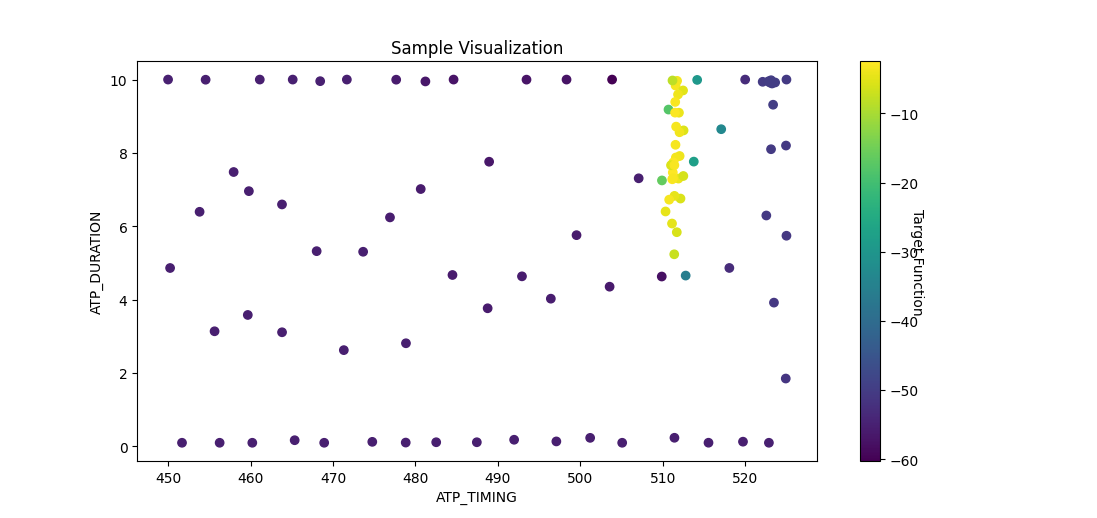
\includegraphics[width = 14cm]{patient_3_attempts.png}
    \caption{impulse timing vs impulse duration for patient 3 with 100 trials. The negative sign of the loss function is justified in Section \ref{alg_t}.}
    \label{patient3attempts}
\end{center}
\end{figure}

\section{Numerical results}
\label{sec:num_results}
\subsection{Results for $\nu_2$}
%\color{red}
Using the algorithm implemented in Section \ref{alg_nu}, we also implement a saving method for each run and each iteration, in order to be capable of finding the best result.\\
In the end, we obtain:
\begin{center}
	\captionof{table}{Optimal $\nu_2$ for each patient}
	\begin{tabular}{|c|c|c|} 
		\hline 
		\rule[-4mm]{0mm}{1cm}
		Patient & $\nu_2$ & MSE \\
		\hline 
		\rule[-4mm]{0mm}{1cm}
		1 & 0.012131080952301447 & 0.020216118044778568 \\
		\hline
		\rule[-4mm]{0mm}{1cm}
		2 &  0.011852260526571526 &
		0.01911400692573191 \\
		\hline 
		\rule[-4mm]{0mm}{1cm}
		3 & 0.01174896977325422 & 0.021651723520038108 \\
		\hline 
	\end{tabular}
\end{center}
We are then compare the exact solution (with noise) and the numerical solution (with the optimal $\nu_2$):
\begin{figure}[H]
\begin{center}
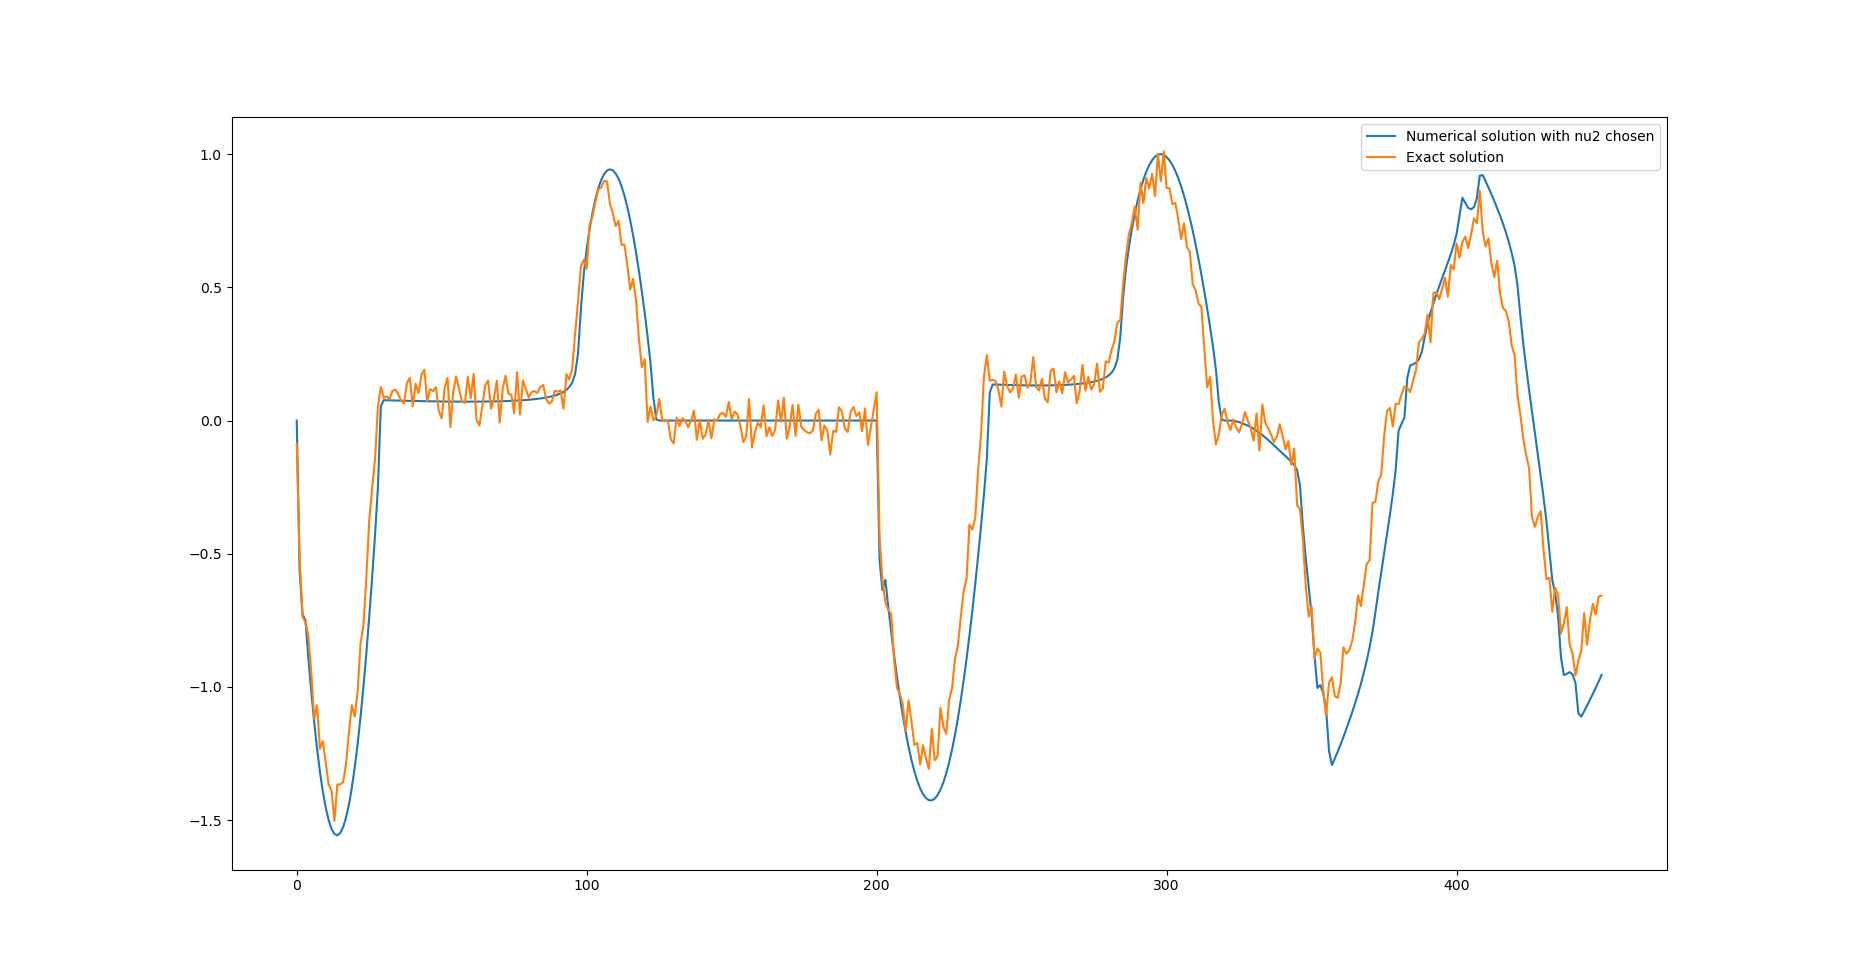
\includegraphics[width = 11cm]{./patient_1_noise.png}
    \caption{Comparison between numerical and exact solutions for the patient 1 with $\nu_2 = 0.012131080952301447$.}
\end{center}
\end{figure}

\begin{figure}[H]
\begin{center}
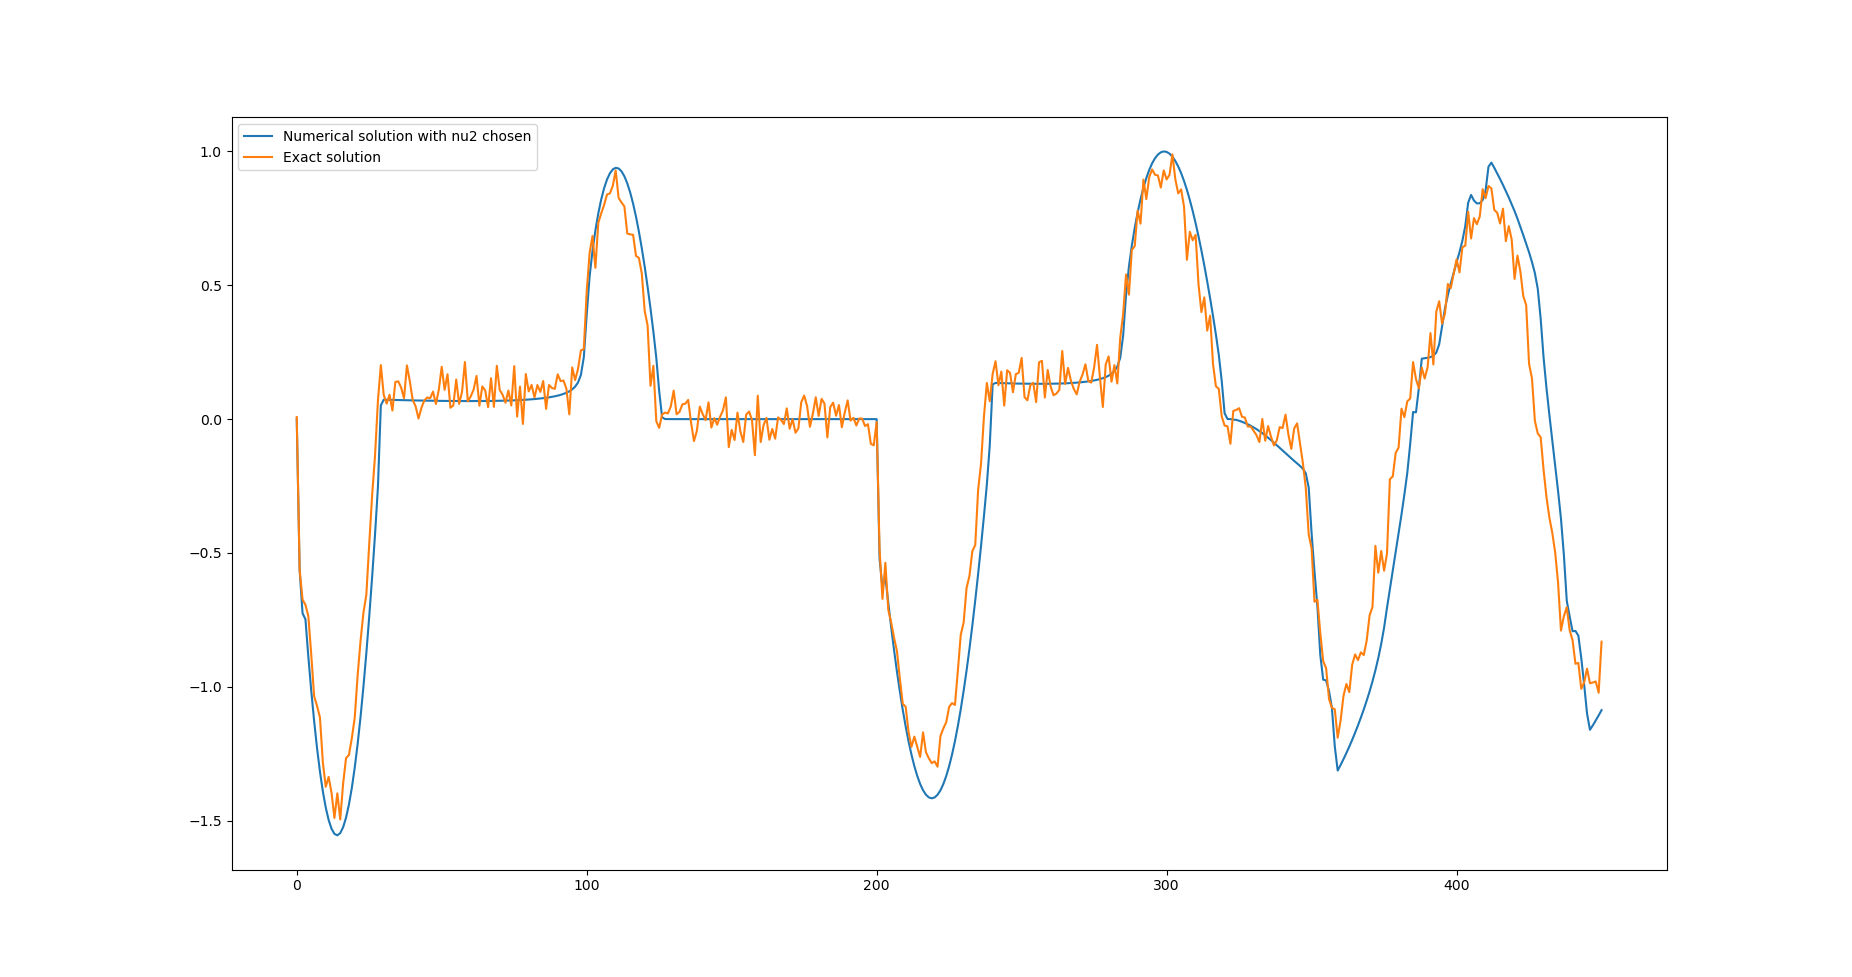
\includegraphics[width = 11cm]{./patient_2_noise.png}
    \caption{Comparison between numerical and exact solutions for the patient 2 with $\nu_2 = 0.011852260526571526$.}
\end{center}
\end{figure}

\begin{figure}[H]
\begin{center}
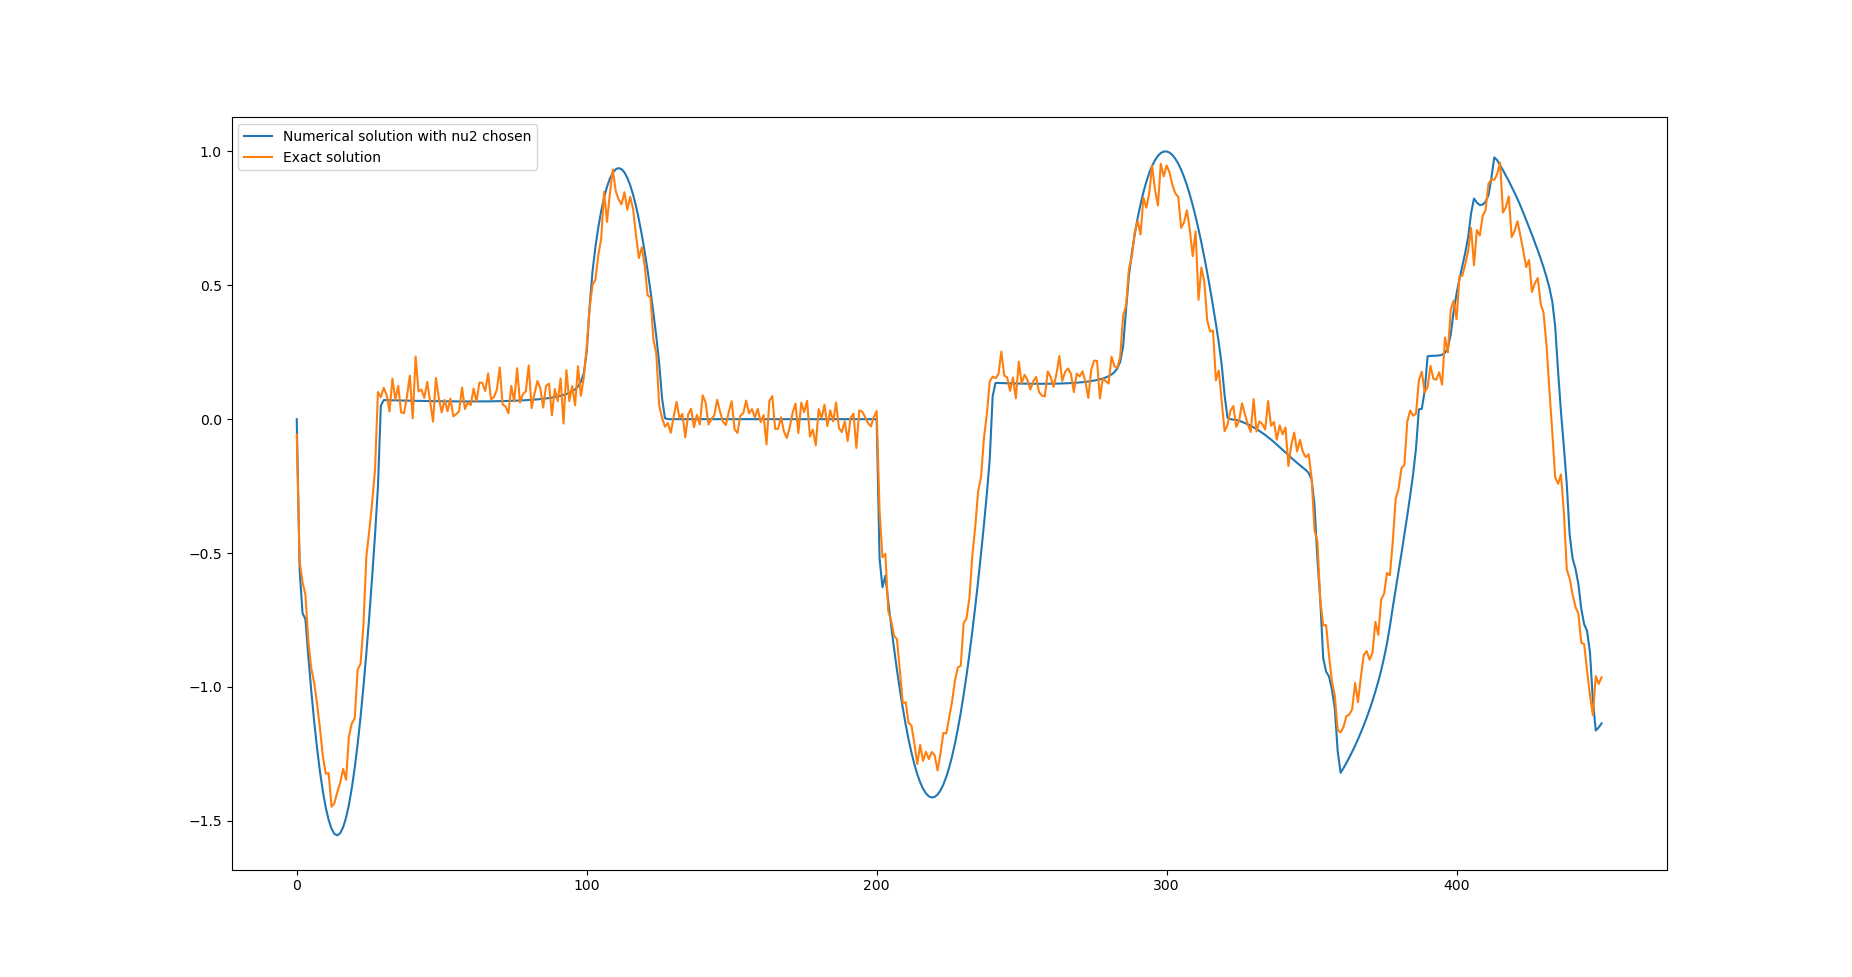
\includegraphics[width = 11cm]{./patient_3_noise.png}
    \caption{Comparison between numerical and exact solutions for the patient 3 with $\nu_2 = 0.01174896977325422$.}
\end{center}
\end{figure}
By plotting the $\nu_2$ parameter and the corresponding MSE reached, we obtain the following plot:
\begin{figure}[H]
\begin{center}
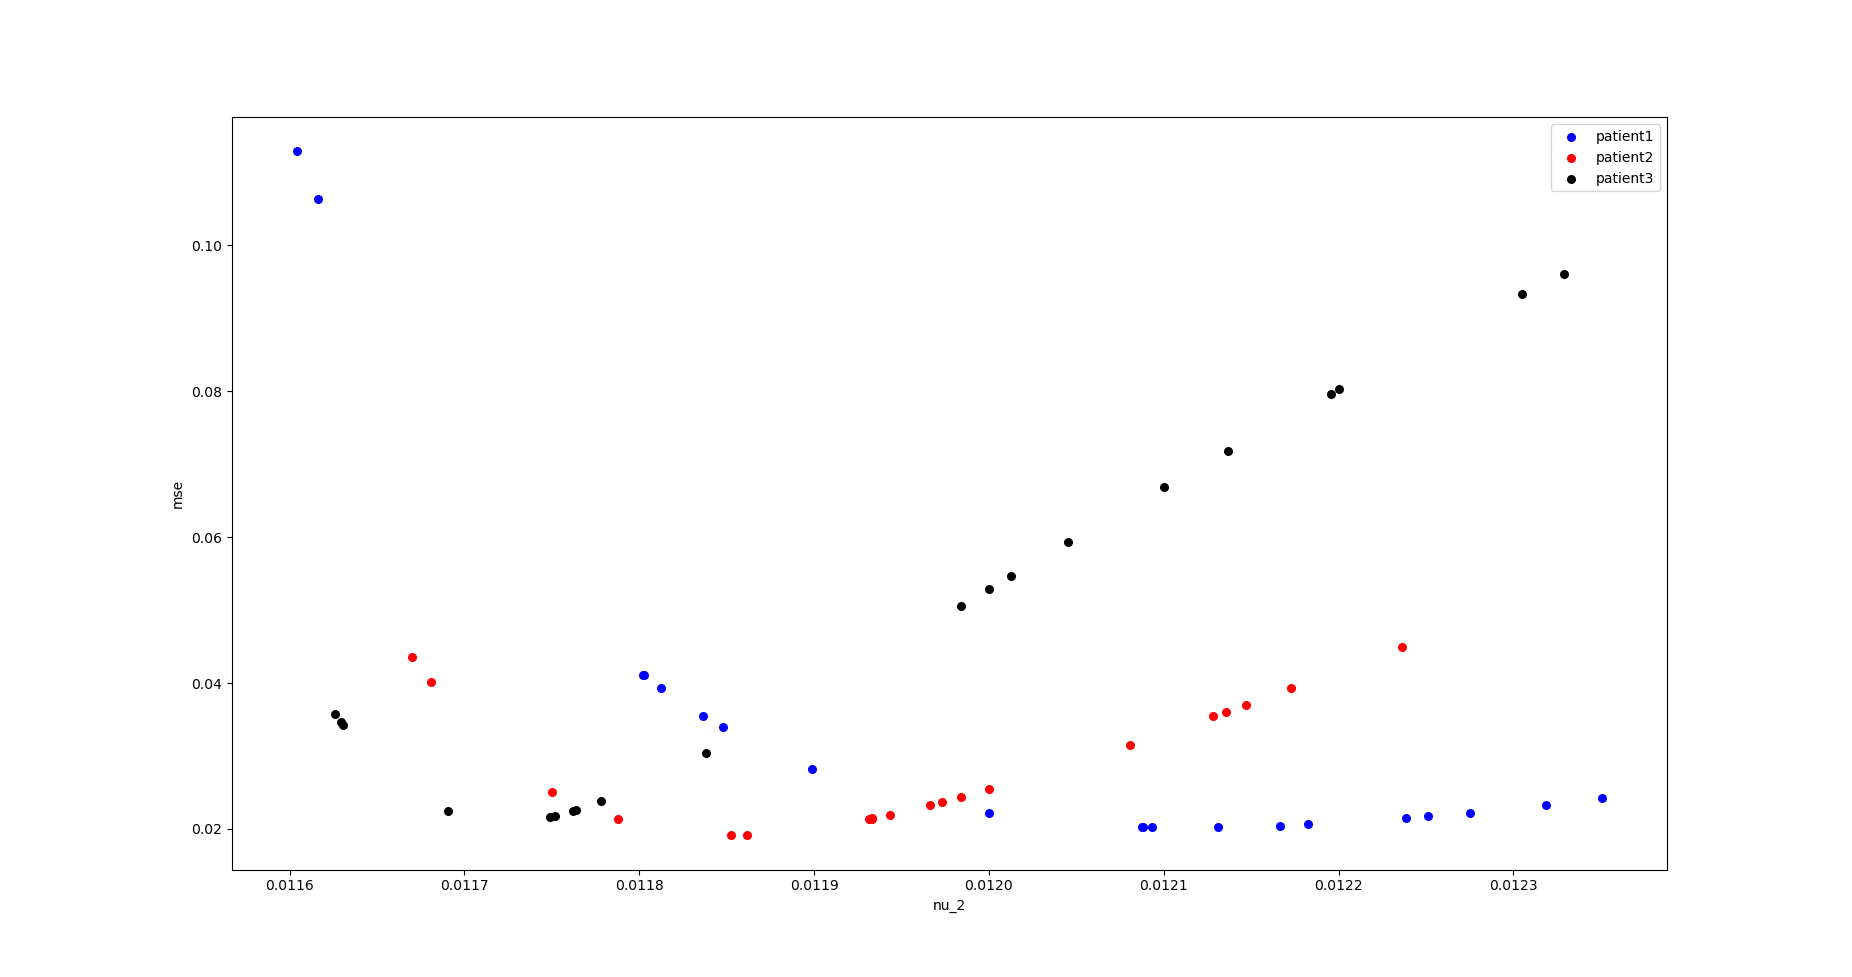
\includegraphics[width = 15cm]{./nu.png}
    \caption{Comparison of different results}
\end{center}
\end{figure}

\subsection{Results for $t_s$ and $\Delta t_s$}
The final values for ATP time and duration for the three patients are:

\begin{itemize}
    \item [P1]: impulse delivered at time 484.707 ms with duration  2.697 ms
    \item [P2]: impulse delivered at time 501.435 ms with duration 2.804 ms
    \item [P3]: impulse delivered at time 511.579 ms with duration 5.038 ms
\end{itemize}
 
The following plots showcase the ability of our impulse strategy to reset the ECG.

\begin{figure}[H]
\begin{center}
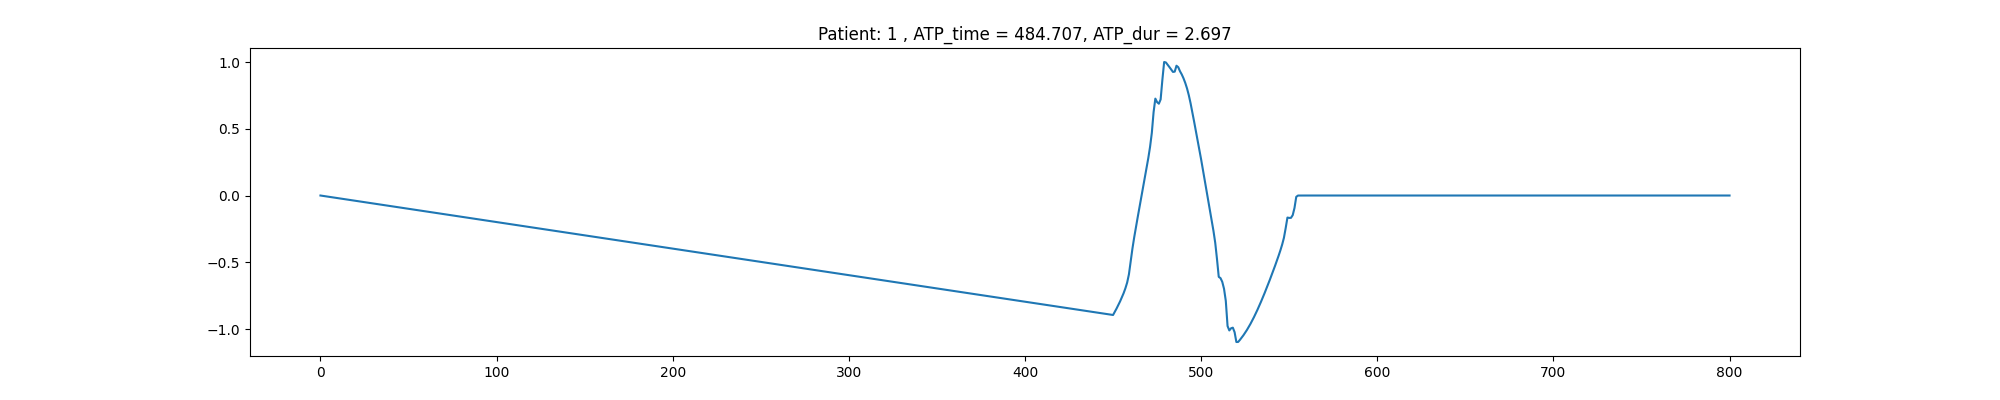
\includegraphics[width = 15cm]{Homework_report/Images/patient_1_ATP_time_484.707_ATP_dur_2.697.png}
    \caption{ECG for patient 1}
    \label{ecgp1}
\end{center}
\end{figure}

\begin{figure}[H]
\begin{center}
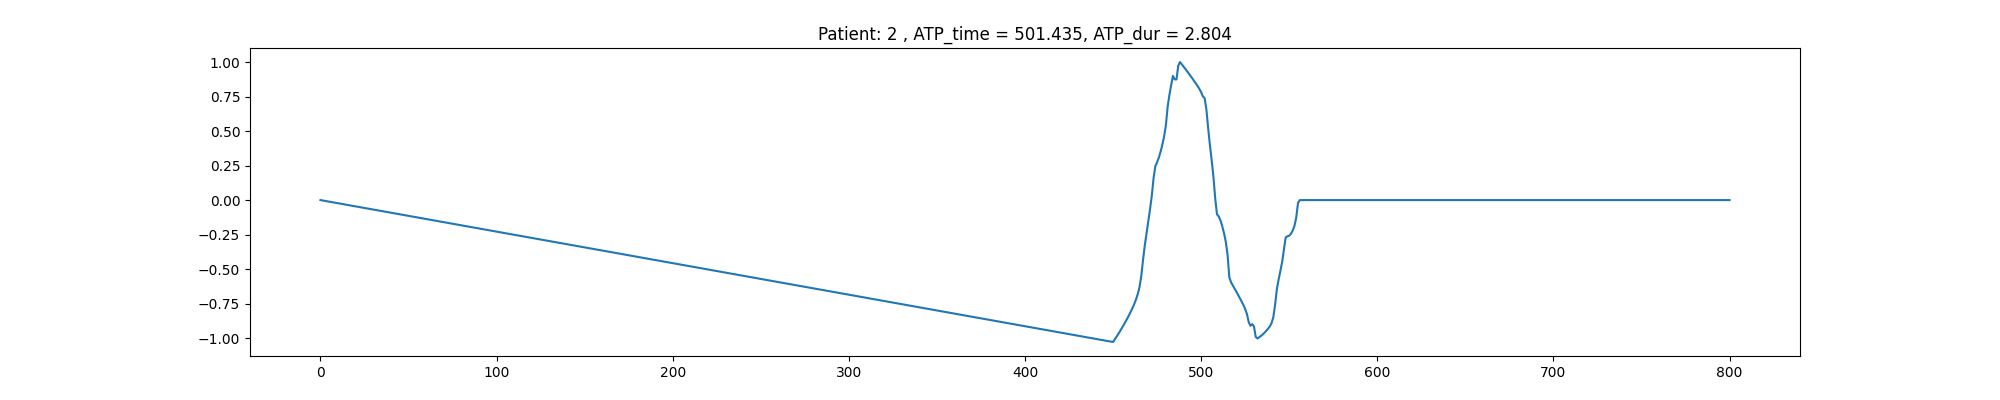
\includegraphics[width = 15cm]{Homework_report/Images/patient_2_ATP_time_501.435_ATP_dur_2.804.png}
    \caption{ECG for patient 2}
    \label{ecgp2}
\end{center}
\end{figure}

\begin{figure}[H]
\begin{center}
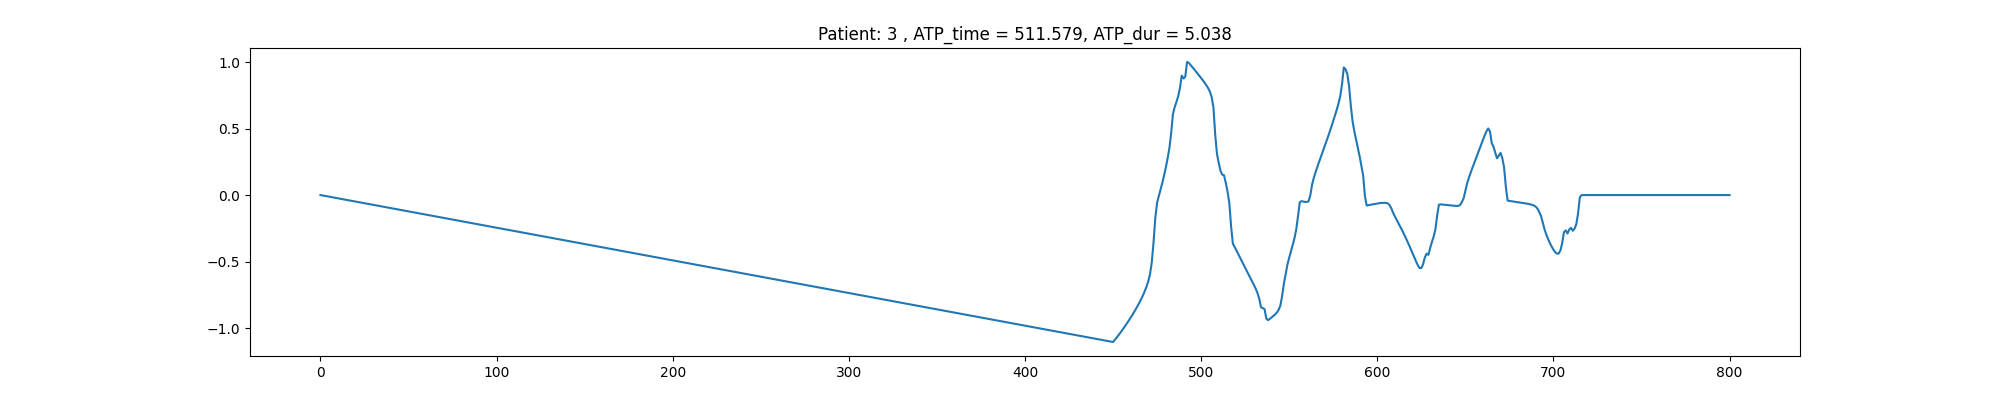
\includegraphics[width = 15cm]{Homework_report/Images/patient_3_ATP_time_511.579_ATP_dur_5.038.png}
    \caption{ECG for patient 3}
    \label{ecgp3}
\end{center}
\end{figure}

Note that for efficiency we saved the initial values of the ECG for the first 450 milliseconds, hence the value plotted until this time instant in Figure \ref{ecgp1}, Figure \ref{ecgp2} and Figure \ref{ecgp3} can be ignored.

\section{Bibliography}
The documentation used to calibrate $\nu_2$ is based on the content of the course, while the documentation for the Bayesian Optimization approach has been taken from \cite{bayesopt_1}, \cite{baysopt_git} and \cite{bayesopt_2}.

%-----------------------------------------------------------------------------
% CONCLUSION
%-----------------------------------------------------------------------------
\section{Conclusions}
Concerning the problem of finding the optimal ATP timing and ATP duration, it is clear from Figure \ref{patient3attempts} that the Bayesian algorithm made lots of attempts in the region of the optimal values and wasted only a few iterations to search for different optimal areas. We are quite satisfied with these results because the computational cost of each iteration was very high and the algorithm effectively exploited the attempts, thus granting an accurate solution after a few iterations.\\
As previously explained, the added feature of a Bayesian Optimization algorithm with respect to a random search, is that it requires a lower number of iterations to propose a point that is close enough to the true argmin of the loss function. Throughout our project, we noticed that the algorithm was able to propose values of impulse timing and duration that would annihilate the ECG in the whole tracking window in just 15 iterations (roughly 30 minutes). \\
Further developments could consider joining the simultaneous estimation of all $\nu_2$, $t_s$ and $\Delta t_s$ parameters in a unique algorithm, because an inaccurate $\nu_2$ parameter could negatively influence the estimation of the other two variables, thus an optimized $\nu_2$ could lead us to obtain an even better result.
%---------------------------------------------------------------------------
%  BIBLIOGRAPHY
%---------------------------------------------------------------------------
% Remember to insert here only the essential bibliography of your work
\bibliography{bibliography.bib} % automatically inserted and ordered with this command

\end{document}
